\section{Robustez} \label{sec:robustez}

Las Tablas \ref{tab:honest_principal} y \ref{tab:honest_mercado} aplican la restricción de magnitudes relativas de \textcite{RAMBACHAN2023}, que reporta el mayor $\bar{M}$ con el que el intervalo robusto excluye el cero, donde $\bar{M} = 1$ significa que la violación posterior a la entrada puede ser tan grande como el mayor salto observado antes de ella. En el primer semestre el efecto sobre el precio de las incumbentes resiste $\bar{M}$ de 1 en la gasolina 93, 1,25 en la 97, 1,75 en la 95 y 2,25 en el diésel, y en el segundo semestre entre 0,75 y 1. En el mercado local el percentil 10 resiste $\bar{M}$ de 1 a 1,75 en el primer semestre, mientras que el percentil 90 no resiste más de 0,75. La tabla del mercado local se estima con TWFE e incluye la versión sin entrante, no el estimador de \textcite{SUNABRAHAM2021} usado en los resultados.

Si la entrada hiciera salir a incumbentes, la caída de precios podría ser un cambio en la composición del mercado y no una respuesta competitiva de las estaciones que se quedan. La Figura \ref{fig:persistencia} estima el efecto de la entrada sobre el número de estaciones a 2 kilómetros o menos. Incluyendo a la entrante el número aumenta en 0,96 estaciones en el primer semestre y se mantiene entre 0,77 y 0,98, por lo que la entrada es un aumento discreto y duradero de la competencia. Excluyendo a la entrante el número de incumbentes no cambia en el primer año (0,03 y 0,05 estaciones menos, no significativo), cuando ya se observa la caída de precios, y baja gradualmente después hasta 0,26 estaciones en el bin $\geq 4$, caída significativa solo en la muestra sin corte en la segunda entrada, por lo que el efecto sobre precios no se explica por la salida de incumbentes.

La Figura \ref{fig:placebo_adelanto} adelanta la fecha de entrada de cada tratada en seis meses, es decir, un bin de la especificación principal. El tiempo se mide en meses desde la entrada registrada para ver dónde ocurre el quiebre, en los cuatro bins a cada lado de ella, con la entrada adelantada en el mes $-6$ y la registrada en el mes 0. En los cuatro combustibles la trayectoria es plana antes de la fecha adelantada y entre ella y la registrada, con una leve caída no significativa en los dos meses previos a la entrada registrada, y el quiebre ocurre en el mes 0, significativo desde ese mes en las gasolinas 93 y 95 y desde el mes 1 en la 97 y el diésel. Esto es consistente con el fechado de la base, y una eventual reacción en el mes previo queda dentro del período de referencia, por lo que el efecto estimado sería una cota inferior.

\begin{figure}[htbp]
    \centering
    \caption{Estudio de eventos con la entrada fechada seis meses antes de la registrada} \label{fig:placebo_adelanto}
    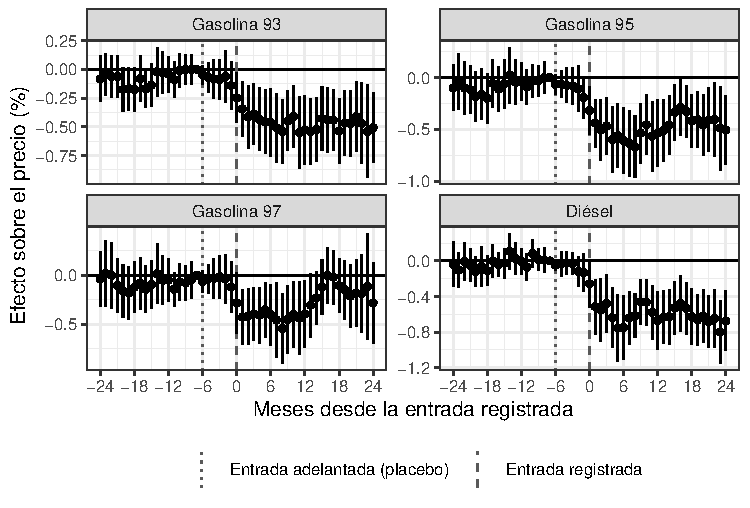
\includegraphics{output/graficos/placebo_adelanto.pdf}
    \caption*{\footnotesize Fuente: Precios históricos de bencinaenlinea.cl. Log del precio $\times$ 100. La fecha de entrada se adelanta un período (seis meses). Tiempo en meses desde la entrada registrada, en los cuatro bins a cada lado de ella, con extremos agrupados en $\pm 24$; la línea punteada marca la entrada adelantada (mes $-6$) y la discontinua la registrada (mes 0). Referencia en el mes previo a la entrada adelantada ($-7$). Misma muestra, efectos fijos (estación, mes, región $\times$ año y marca $\times$ año) y control que la especificación principal. Intervalos al 95\% con errores estándar agrupados por comuna.}
\end{figure}

La Tabla \ref{tab:placebo_controles} asigna fechas de entrada falsas a estaciones del grupo de control, con la misma proporción de tratadas y la misma distribución de cohortes que la muestra real, y estima el efecto 500 veces sobre todo el grupo y sobre su mitad más densa. El efecto placebo promedio está entre 0,00\% y 0,02\%, frente a efectos reales de 0,24\% a 0,59\%, por lo que el diseño no genera efectos donde no hay entrada. Los errores agrupados por comuna son similares a la dispersión efectiva de los placebos en todo el grupo y cerca de 10\% menores en la mitad densa, con tasas de rechazo al 5\% de entre 4\% y 7\% y de hasta 8\%, respectivamente. El valor $p$ por aleatorización del efecto real es de 0,002 o menos en las gasolinas 93 y 95 y el diésel, y en la gasolina 97 de 0,03 en todo el grupo y 0,07 en la mitad densa.

\begin{figure}[htbp]
    \centering
    \caption{Efecto de la entrada sobre el precio de las incumbentes, ventana 2014 a 2019} \label{fig:ventana_2014_2019}
    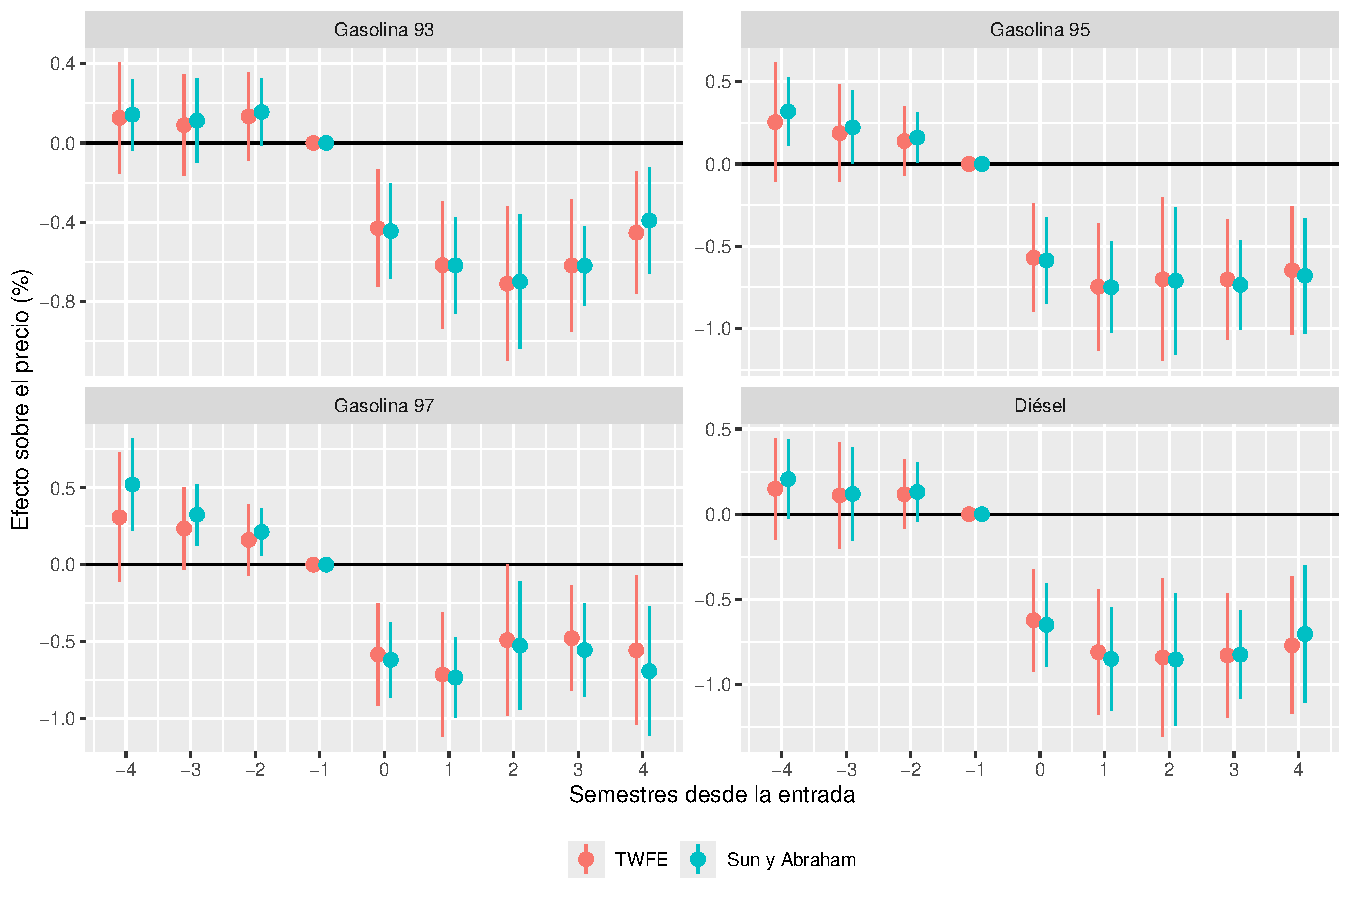
\includegraphics{output/graficos/ventana_2014_2019.pdf}
    \caption*{\footnotesize Fuente: Precios históricos de bencinaenlinea.cl. Incumbentes presentes en 2014 y cohortes de entrada de 2015 a 2019. Log del precio $\times$ 100. Eje horizontal en semestres: bins de seis meses desde la entrada, extremos agrupados, referencia en $-1$. Efectos fijos de estación, mes, región $\times$ año y marca $\times$ año. \textcite{SUNABRAHAM2021} con cohortes mensuales y las nunca tratadas como referencia. Intervalos al 95\% con errores estándar agrupados por comuna. Control: estaciones sin entradas a menos de 5 km. Entre 418 y 459 tratadas y entre 557 y 697 controles según el combustible.}
\end{figure}

\begin{figure}[htbp]
    \centering
    \caption{Efecto de la entrada sobre el precio de las incumbentes, ventana 2021 a 2026} \label{fig:ventana_2021_2026}
    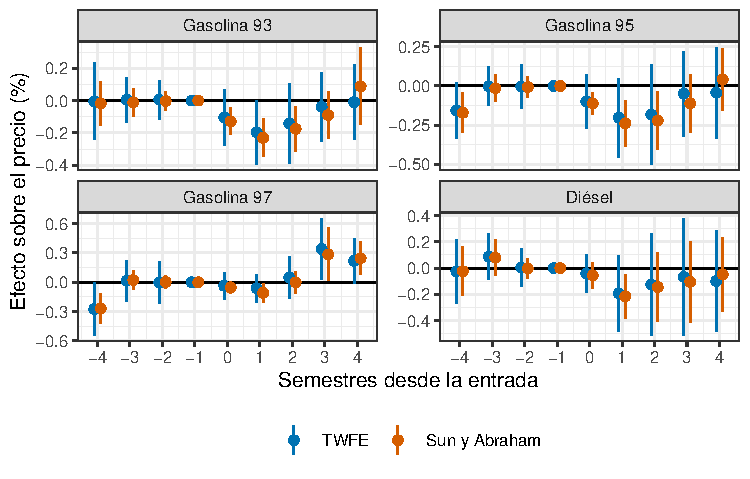
\includegraphics{output/graficos/ventana_2021_2026.pdf}
    \caption*{\footnotesize Fuente: Precios históricos de bencinaenlinea.cl. Incumbentes presentes en 2021 y cohortes de entrada de 2022 a febrero de 2026. Log del precio $\times$ 100. Eje horizontal en semestres: bins de seis meses desde la entrada, extremos agrupados, referencia en $-1$. Efectos fijos de estación, mes, región $\times$ año y marca $\times$ año. \textcite{SUNABRAHAM2021} con cohortes mensuales y las nunca tratadas como referencia. Intervalos al 95\% con errores estándar agrupados por comuna. Control: estaciones sin entradas a menos de 5 km. Entre 180 y 199 tratadas y entre 1.025 y 1.194 controles según el combustible.}
\end{figure}

Las Figuras \ref{fig:ventana_2014_2019} y \ref{fig:ventana_2021_2026} repiten el estudio de eventos principal con TWFE y \textcite{SUNABRAHAM2021} en las ventanas antes y después de la pandemia, y las Tablas \ref{tab:ventana_2014_2019} y \ref{tab:ventana_2021_2026} reportan los coeficientes. Antes de la pandemia el efecto es mayor que en la ventana completa: el precio cae entre 0,43\% (gasolina 93) y 0,62\% (diésel) en el primer semestre y hasta 0,84\% en el diésel, con ambos estimadores prácticamente iguales. Los bins previos son positivos en los cuatro combustibles, entre 0,09\% y 0,31\% con TWFE y no significativos salvo el bin $-3$ de la gasolina 97 al 10\%, pero con \textcite{SUNABRAHAM2021} son significativos en las gasolinas 95 y 97, por lo que en esta ventana los precios ya venían cayendo antes de la entrada y parte del efecto podría reflejar esa tendencia. Aun así, los bins previos son menores que los efectos posteriores en todos los combustibles.



Después de la pandemia el efecto es menor y dura menos. En las gasolinas 93 y 95 el precio cae entre 0,11\% y 0,24\% en los tres primeros semestres con \textcite{SUNABRAHAM2021} y deja de ser distinguible de cero desde el cuarto, en el diésel la caída es de 0,22\% solo en el segundo semestre, y en la gasolina 97 no hay un efecto negativo persistente y los bins 3 y $\geq 4$ son positivos. Con TWFE los puntos estimados son parecidos pero casi ningún coeficiente es significativo, dado que la ventana tiene menos de 200 tratadas, y los intervalos de \textcite{SUNABRAHAM2021} son más angostos. Los bins previos son cercanos a cero salvo el bin $-4$ de las gasolinas 95 y 97, por lo que la debilidad del efecto no se explica por tendencias previas.
